\chapter{Rock Paper Scissors}
\label{RPS}
\graphicspath{ {./Lab03RockPaperScissor/Fig} }


\section{Outcomes and Objectives}

The outcome of this lab is to instantiate a rock, paper scissors games
on the FPGA development board. 
Through this process you will achieve the following
learning objectives.
\begin{itemize}
	\itemsep=0em
	\item \Paste{bok:REP_WordStatement}
	\item \Paste{bok:REP_TruthTable}
	\item \Paste{VER:CSA}
	\item \Paste{VER:Module}
	\item \Paste{VER:Instantiating}
	\item \Paste{HDL:Pin}
	\item \Paste{HDL:Synthesis}
\end{itemize}

\section{The Rock Paper Scissors Game}

The game of rock, paper, scissors is a two-player game whose goal is to
beat the throw of the opposing player. Traditionally, each player throws
one of three plays, rock, paper, or scissors by extending their hand in
the shape of the object.

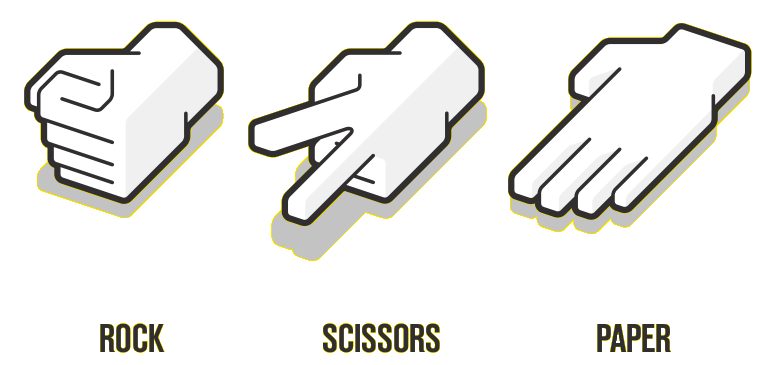
\includegraphics[width=0.4\paperwidth]{ image1.png}

The rules of the game state that:

\begin{tabular}{p{4cm}p{4cm}p{4cm}}
Rock beats scissors  & Scissors beats paper & Paper beats rock \\
\end{tabular}

Since prior knowledge of your opponent's throw would provide an unfair
advantage, the two players make their throws at the same time. Your goal 
in this lab is to create a digital version of rock, paper,
scissors on the Altera Cyclone V Board using the inputs and outputs
shown in Figure~\ref{figure:systemIO}. Each player will have access to three slide switches
and one 7-segment display. Each of the three switches represents one of
the three plays and the 7-segment will display the throw when the Play
button is pressed. The Win/Lose 7-segment display will show ``1'' when
player 1 wins, ``2'' when player 2 wins, and ``d'' when the game is a
draw (a tie).

\begin{figure}[ht]
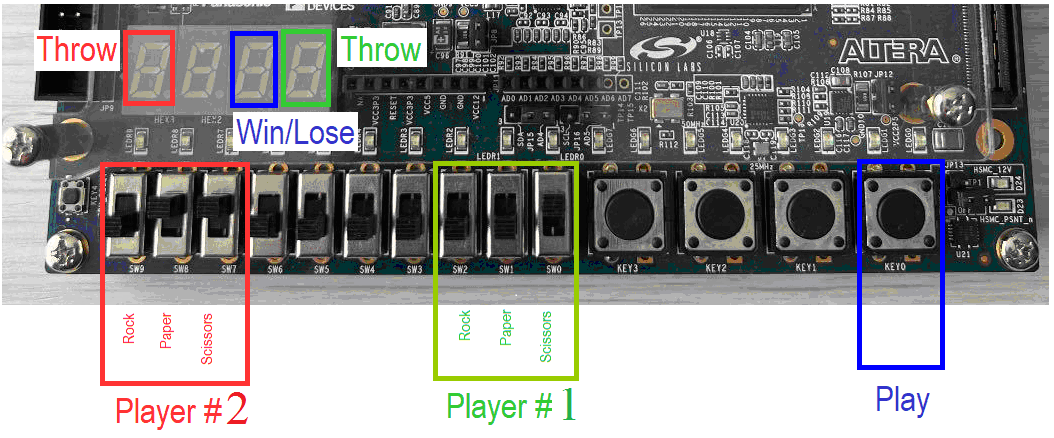
\includegraphics{ image2.png}
\caption{The input and output you should use to realize your digital system.}
\label{figure:systemIO}
\end{figure}



A player will move one of the three slides-switches into the up position
to indicate their play. Moving more than one slide-switch, or no slide
switch into the up position is in an invalid play. An invalid play
always loses to a valid play. If each player throws an invalid play, the
game is a draw.

While each player is making their choice of play, their Throw 7-segment
display will reflect their choice as shown in Figure~\ref{figure:play7seg}. These patterns
are supposed to vaguely resemble the objects.

\begin{figure}[ht]
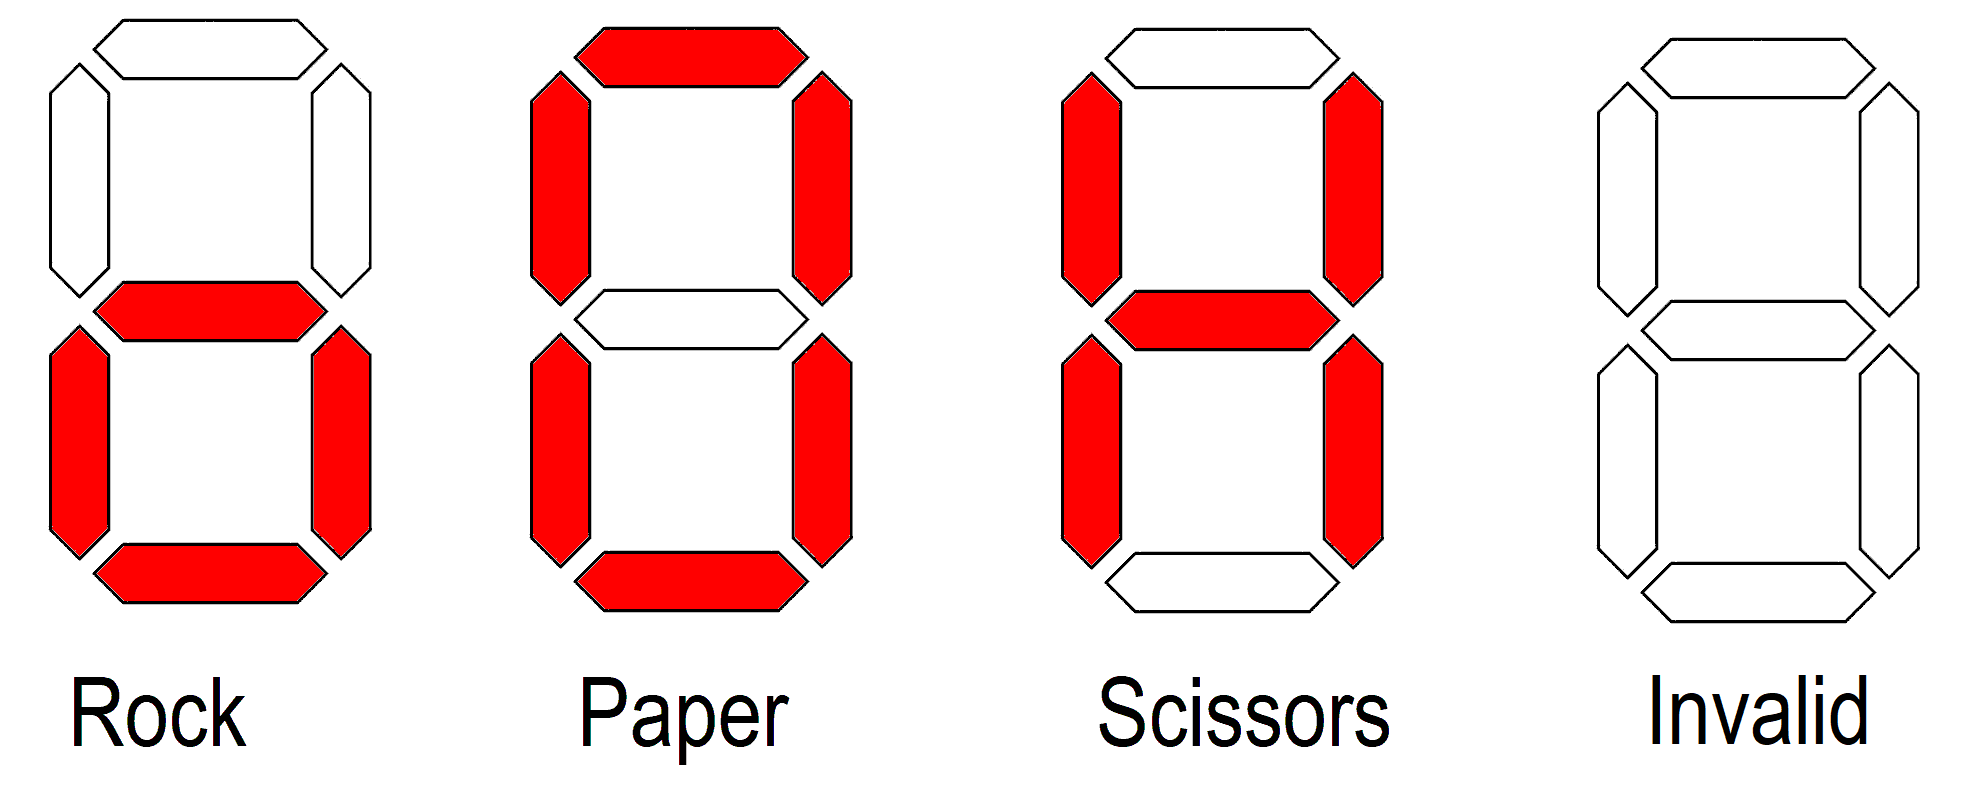
\includegraphics[width=0.3\paperwidth]{image3.png}
\caption{Illuminated patters for the different plays.}
\label{figure:play7seg}
\end{figure}

When the Throw button is pressed, the Win/Lose 7-segment will display
``1'', ``2'', or ``d'' depending on the outcome of the game as shown in
Table~\ref{table:gameLogic}. When the Throw button is un-pressed, the Win/Lose 7-segment
display is blank.

\begin{longtable}[]{@{}
| >{\raggedright\arraybackslash}p{(\columnwidth - 8\tabcolsep) * \real{0.1999}}|
  >{\raggedright\arraybackslash}p{(\columnwidth - 8\tabcolsep) * \real{0.2000}}|
  >{\raggedright\arraybackslash}p{(\columnwidth - 8\tabcolsep) * \real{0.2000}}|
  >{\raggedright\arraybackslash}p{(\columnwidth - 8\tabcolsep) * \real{0.2000}}|
  >{\raggedright\arraybackslash}p{(\columnwidth - 8\tabcolsep) * \real{0.2000}}|@{}}
\caption{The output for every combination of player 1 (P1) and player 2 (P2) throws.}  
\label{table:gameLogic}
\tabularnewline
\toprule()
\begin{minipage}[b]{\linewidth}\raggedright
P1 \textbackslash{} P2
\end{minipage} & \begin{minipage}[b]{\linewidth}\raggedright
Rock
\end{minipage} & \begin{minipage}[b]{\linewidth}\raggedright
Paper
\end{minipage} & \begin{minipage}[b]{\linewidth}\raggedright
Scissors
\end{minipage} & \begin{minipage}[b]{\linewidth}\raggedright
Invalid
\end{minipage} \\ \hline
\midrule()
\endfirsthead
\toprule()
\begin{minipage}[b]{\linewidth}\raggedright
P1 \textbackslash{} P2
\end{minipage} & \begin{minipage}[b]{\linewidth}\raggedright
Rock
\end{minipage} & \begin{minipage}[b]{\linewidth}\raggedright
Paper
\end{minipage} & \begin{minipage}[b]{\linewidth}\raggedright
Scissors
\end{minipage} & \begin{minipage}[b]{\linewidth}\raggedright
Invalid
\end{minipage} \\\hline
\midrule()
\endhead
Rock & d & 2 & 1 & 1 \\ \hline
Paper & 1 & d & 2 & 1 \\ \hline
Scissors & 2 & 1 & d & 1 \\ \hline
Invalid & 2 & 2 & 2 & d \\ \hline

\end{longtable}

\section{System Architecture}
The system architecture shown in Figure~\ref{fig:sysArch} is your guide to building
a functioning circuit. As such, we will take a moment to cover some important
details of this diagram that will help you write your Verilog code later./

The names outside
the FPGA square correspond to the labels in Figure~\ref{figure:systemIO}. Each soft-square
(a square with rounded corners) is a Verilog module. Names inside
soft-squares, that are adjacent to lines outside the soft-square, are
the port names for that module. The instance name and module name of a
module are separated by a ``:'' and usually located along the top edge
of the soft-square. Red soft-squares are associated with player 1 and
green soft-squares associated with player 2. The names on lines inside
the rpsGame soft-square are the signals names you should use in the
rpsGame module to connect the 5 modules together. Lines that are slashed
with a number denote bit vectors.

\begin{figure}[ht]
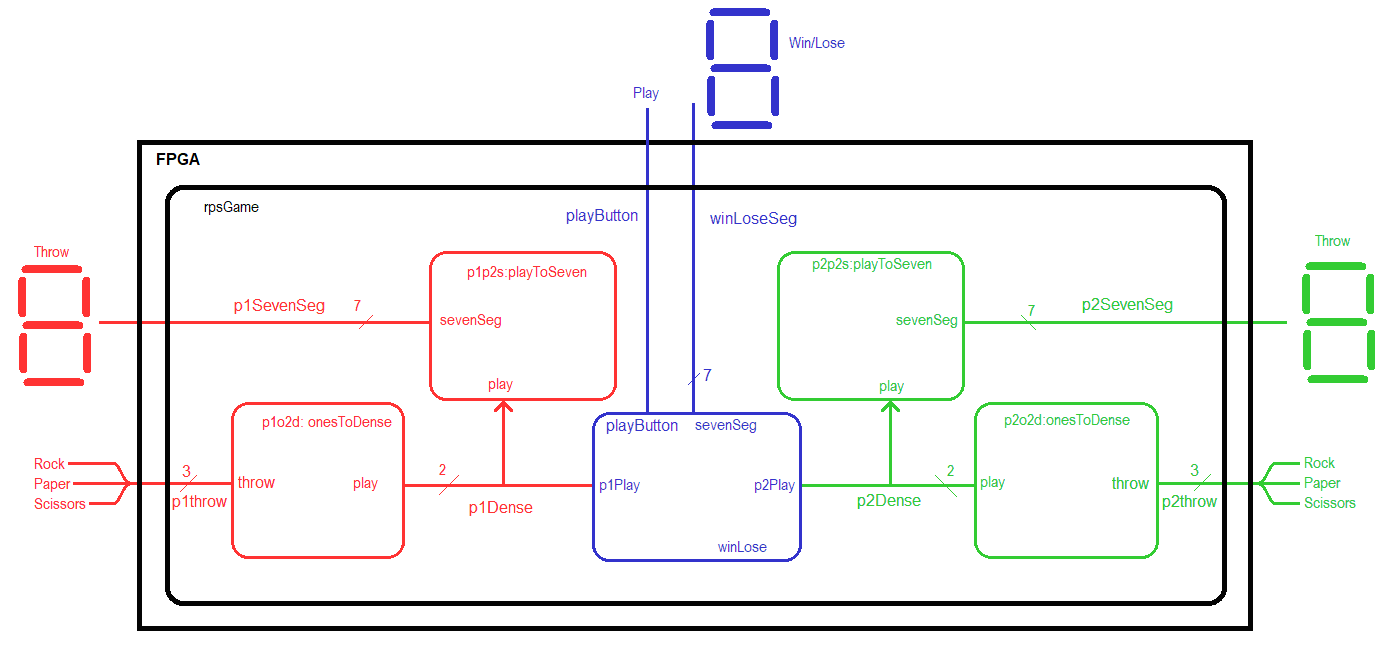
\includegraphics{ image4.png}
\caption{System architecture for the rock, paper, scissors system.}
\label{fig:sysArch}
\end{figure}

\hypertarget{onestodense-module}{%
\section{Module: onesToDense}
\label{onestodense-module}}

Each player makes their throw selection by placing one of the three
slide switches into the up position. As a result of this game mechanic,
there are only three valid input combinations for the rock, paper,
scissors trio. These are:

\begin{itemize}
\item
  (1,0,0) for when the player moves only the rock slide switch up,
\item
  (0,1,0) for when the player moves only the paper slide switch up,
\item
  (0,0,1) for when the player moves only the scissor slide switch up.
\end{itemize}

Having a code where only one of the bits is equal logic 1 is called a
``ones-hot'' code. The ``hot'' bit being logic 1. A code where every
possible combination of bits is assigned a meaning is called a dense
code.

This module will convert the input ones-hot code into a dense code. In
order to correctly determine the outcome of the game, we need to know
when the user has entered an invalid play; the output of this module
must be able to represent \{rock, paper, scissors, invalid\}. You will
encode these four combinations in 2-bits as \{2'b00, 2b'01, 2'b10,
2'b11\} respectively.

In order to write the Verilog code for this module, complete the truth
table in Table~\ref{table:onesToDense} for the onesToDense module.

\begin{itemize}
\item
  r is the state of the rock slide-switch. r=0 slide switch is down. r=1
  slide-switch up.
\item
  p is the state of the paper slide-switch. p=0 slide switch is down.
  p=1 slide-switch up
\item
  s is the state of the scissor slide-switch. s=0 slide switch is down.
  s=1 slide-switch up
\item
  play = \{00\} means rock was selected
\item
  play = \{01\} means paper was selected
\item
  play = \{10\} means scissor was selected
\item
  play = \{11\} means invalid selection was made
\end{itemize}

\begin{longtable}[]{@{}
| >{\raggedright\arraybackslash}p{(\columnwidth - 8\tabcolsep) * \real{0.1999}}|
  >{\raggedright\arraybackslash}p{(\columnwidth - 8\tabcolsep) * \real{0.2000}}|
  >{\raggedright\arraybackslash}p{(\columnwidth - 8\tabcolsep) * \real{0.2000}}|
  >{\raggedright\arraybackslash}p{(\columnwidth - 8\tabcolsep) * \real{0.2000}}|
  >{\raggedright\arraybackslash}p{(\columnwidth - 8\tabcolsep) * \real{0.2000}}|@{}}
\caption{The truth table for the onesToDense module.}\label{table:onesToDense}\tabularnewline 
\toprule()
r & p & s & play & Note \\ \hline
\midrule()
\endfirsthead
\toprule()
r & p & s & play & Note \\ \hline
\midrule()
\endhead
0 & 0 & 0 & & \\ \hline
0 & 0 & 1 & & \\ \hline
0 & 1 & 0 & & \\ \hline
0 & 1 & 1 & & \\ \hline
1 & 0 & 0 & 00 & Rock \\ \hline
1 & 0 & 1 & & \\ \hline
1 & 1 & 0 & & \\ \hline
1 & 1 & 1 & & \\ \hline
\end{longtable}

From this truth table, determine the canonical SOP expressions for
play{[}1{]} and play{[}0{]} functions. Do this by writing the canonical
SOP expression for the most significant bit of the play output,
play{[}1{]}, in the Table~\ref{table:onesToDense} truth table while ignoring the LSB. Then
proceed to write the canonical SOP expression for the LSB of the play
output, play{[}0{]}, in the Table~\ref{table:onesToDense} truth table while ignoring the MSB.

\protect\hypertarget{ones2Dense_CanonicalSOP}{}{}play{[}1{]} =

play{[}0{]} =

\protect\hypertarget{ones2Dense_Verilog}{}{}Now it's time to write the
Verilog code. Incorporate the following into your onesToDense Verilog
module:

\begin{itemize}
\item
  Use the module declaration: module onesToDense (throw, play);
\item
  Use vectors for the throw input. The MSB should come from the rock
  slide-switch and the LSB from the scissors slide-switch.
\item
  Use a vector for the play output.
\item
  Make the input and output port types ``wire''.
\item
  You may want to break the input vector into its component pieces to
  correspond to the variable names used in Table~\ref{table:onesToDense}.
   This will require
  a wire declaration and two assign statements to give each variable
  1-bit from the input vector.
\item
  Use assign statements to realize the AND, OR, NOT logic derived for
  your canonical SOP expressions.
\item
  Use function04 from lab 1 as a starting point for this module.
\end{itemize}

\hypertarget{playtoseven-module}{%
\section{Module: playToSeven}
\label{playtoseven-module}}

The playToSeven module converts the player throw, represented in the
dense coding, to a ``graphical'' form displayed on the 7-segment
display. The symbols for each possible throw are shown in Figure~\ref{figure:throw7seg}.

\begin{figure}[ht]
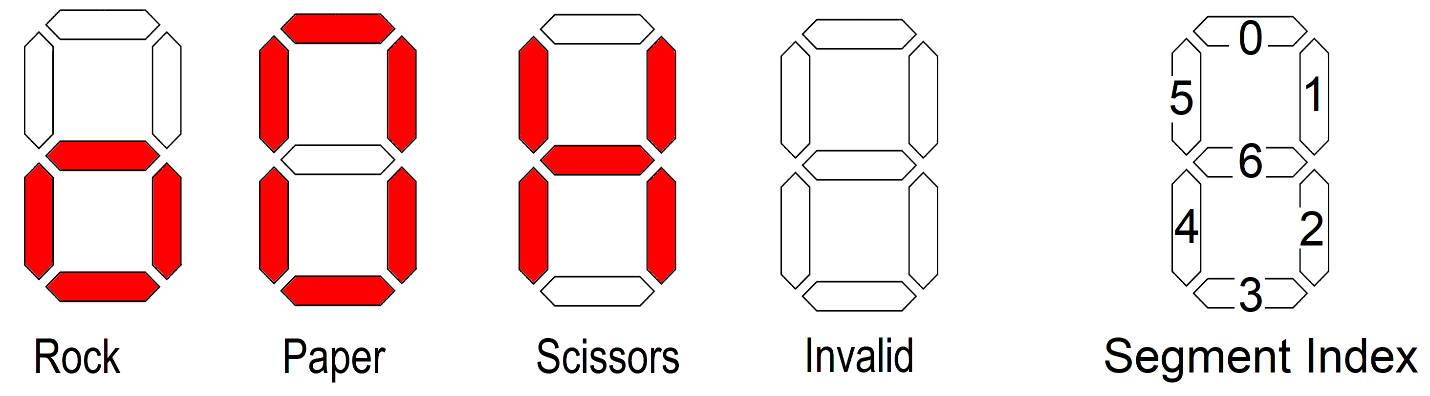
\includegraphics{ image5.png}
\caption{7-segment display patterns for the different throws along with
the 7-segment display segment indices.}
\label{figure:throw7seg}
\end{figure}

Use the information in Figure~\ref{figure:throw7seg} to determine the bit patterns needed to
generate the four different symbols in Table~\ref{table:throwSevenSeg}. Remember that the LEDs
in the segments are active low, meaning that a logic 0 output
illuminates an LED segment. In Table~\ref{table:throwSevenSeg} put a 0 or 1 in each of the
numbered column so that each row produces the patterns for its throw.
Remember that pPlay codes rock as 00, paper as 01, scissors as 10 and an
invalid throw is coded as 11. In the sevenSeg column put the 7-bit code
formed by concatenating the bits together. Use proper Verilog syntax to
write this 7-bit vector.

\begin{longtable}[]{@{}
| >{\raggedright\arraybackslash}p{(\columnwidth - 18\tabcolsep) * \real{0.1513}}|
  >{\raggedright\arraybackslash}p{(\columnwidth - 18\tabcolsep) * \real{0.0643}}|
  >{\raggedright\arraybackslash}p{(\columnwidth - 18\tabcolsep) * \real{0.0643}}|
  >{\raggedright\arraybackslash}p{(\columnwidth - 18\tabcolsep) * \real{0.0643}}|
  >{\raggedright\arraybackslash}p{(\columnwidth - 18\tabcolsep) * \real{0.0643}}|
  >{\raggedright\arraybackslash}p{(\columnwidth - 18\tabcolsep) * \real{0.0643}}|
  >{\raggedright\arraybackslash}p{(\columnwidth - 18\tabcolsep) * \real{0.0643}}|
  >{\raggedright\arraybackslash}p{(\columnwidth - 18\tabcolsep) * \real{0.0643}}|
  >{\raggedright\arraybackslash}p{(\columnwidth - 18\tabcolsep) * \real{0.2210}}|
  >{\raggedright\arraybackslash}p{(\columnwidth - 18\tabcolsep) * \real{0.1777}}|@{}}
\caption{The 7-segment display LEDs to produce the throw patterns.}\label{table:throwSevenSeg}\tabularnewline
\toprule()
pPlay & 6 & 5 & 4 & 3 & 2 & 1 & 0 & sevenSeg & Note \\ \hline
\midrule()
\endfirsthead
\toprule()
pPlay & 6 & 5 & 4 & 3 & 2 & 1 & 0 & sevenSeg & Note \\ \hline
\midrule()
\endhead
00 & & & & & & & & & Rock \\ \hline
01 & & & & & & & & & Paper \\ \hline
10 & & & & & & & & & Scissors \\ \hline
11 & & & & & & & & 7'b1111111 & Invalid \\
\bottomrule()
\end{longtable}

\protect\hypertarget{play2Seven_Verilog}{}{}Incorporate the following
into your playToSeven Verilog module:

\begin{itemize}
\item
  Use the module declaration: \verb+module playToSeven (pPlay, sevenSeg);+
\item
  Use a vector for the input pPlay and a vector for the sevenSeg output.
\item
  Make the input port type ``wire''. Make the output port type ``reg''.
\item
  Use a case statement, embedded in an always statement to realize this
  module. Enumerate all combinations of the input; do not use a default
  case
\item
  Use the information in Table~\ref{table:throwSevenSeg} to assign values to the output.
\item
  Put comments at the end of each case row describing, in words, what
  the output should look like on the 7-segment display.
\item
  Use the hex2Seven module from lab 2 as the starting point for this
  module.
\end{itemize}


\section{Module: winLose}

The winLose module takes the throw from each player (in the dense
coding), the push button, and determines what to display on the win/lose
7-segment display. The win/lose 7-segment display is blank when the
button is not being pressed, otherwise it will show ``1'' when player 1
has a winning throw, ``2'' when player two has the winning throw, ``d''
when the players have the same throw. The patterns are the same as those
you have already created for the hexToSeven module and are shown in
Figure~\ref{fig:winLose7seg} as a reminder.

\begin{figure}[ht]
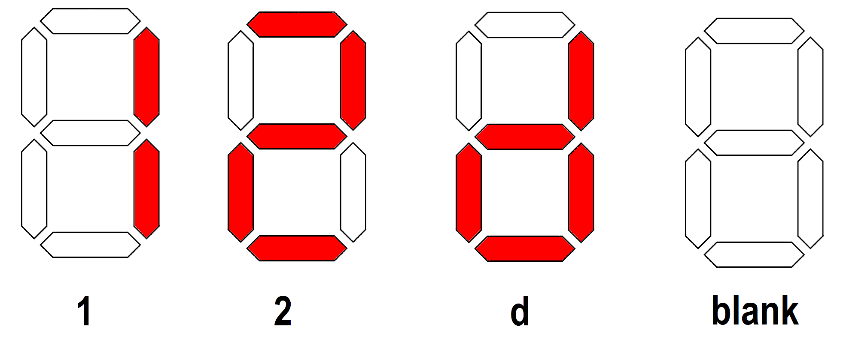
\includegraphics{ image6.png}
\caption{The illuminated patterns displayed on the win/lose 7-segment display.}
\label{fig:winLose7seg}
\end{figure}

You will use a case statement, based on the information in Table~\ref{table:winLooseTt}, to
realize this function. In the sevenSeg column put the 7-bit code needed
to illuminate the winLose 7-segment display to indicate the outcome of
the game. In the Note column put either ``1'', ``2'', ``Draw'', or
``Blank'' depending on the outcome of the game and button press. Use the
bit order given in Figure~\ref{figure:throw7seg}.

\begin{longtable}[]{@{}
| >{\raggedright\arraybackslash}p{(\columnwidth - 8\tabcolsep) * \real{0.1723}}|
  >{\raggedright\arraybackslash}p{(\columnwidth - 8\tabcolsep) * \real{0.2093}}|
  >{\raggedright\arraybackslash}p{(\columnwidth - 8\tabcolsep) * \real{0.2055}}||
  >{\raggedright\arraybackslash}p{(\columnwidth - 8\tabcolsep) * \real{0.2188}}|
  >{\raggedright\arraybackslash}p{(\columnwidth - 8\tabcolsep) * \real{0.1941}}|@{}}
\caption{Abbreviated truth table for the winLose module.}\label{table:winLooseTt}\tabularnewline
\toprule()

button & p1Play & p2Play & sevenSeg & Note \\ \hline
\midrule()
\endfirsthead
\toprule()
button & p1Play & p2Play & sevenSeg & Note \\ \hline
\midrule()
\endhead
0 & & & & \\ \hline
0 & & & & \\ \hline
0 & & & & \\ \hline
0 & & & & \\ \hline
0 & & & & \\ \hline
0 & & & & \\ \hline
0 & & & & \\ \hline
0 & & & & \\ \hline
0 & 10 (scissors) & 00 (rock) & 7'b0100100 & 2 \\ \hline
0 & & & & \\ \hline
0 & & & & \\ \hline
0 & & & & \\ \hline
0 & & & & \\ \hline
0 & & & & \\ \hline
0 & & & & \\ \hline
0 & & & & \\ \hline
1 & xx (don't care) & xx (don't care) & 7'b1111111 & Blank \\
\bottomrule()
\end{longtable}

\protect\hypertarget{winLoose_Verilog}{}{}Incorporate the following into
your winLose Verilog module: Use the module and port names given in
Figure~\ref{fig:sysArch}.

\begin{itemize}
\item
  Use the module declaration:
\verb+ module winLose(p1Play, p2Play, playButton, sevenSeg);+

\item
  Use vectors for the p1Play and p2Play inputs.
\item
  Use a vector for the sevenSeg output.
\item
  Make the input port types ``wire''. Make the output port types  ``reg''.

\item
  You will use a case statement, embedded in an always statement to
  realize this module.

  \begin{itemize}
  \item
    Use brackets to make the vector for the case statement. For example,
    if button was a 1-bit signal and play was a 2-bit signal, then
    
\begin{lstlisting}[language=Verilog, frame=single]
case ({button, play})
    3'b000:  seg = 7'b1000000;    // display ``0''
    3'b001:  seg = 7'b1111001;    // display ``1''
    3'b010:   seg = 7'b0100100;    // display ``2''
    3'b011:   seg = 7'b0110000;    // display ``3''
    default:  seg = 7'b1111111;    // blank 7-seg
endcase
    \end{lstlisting}
    
  \end{itemize}

This code snippet will use the 3-bit value (button as MSB and play as
least significant 2-bits) to select one of the rows. Note that the
default case handles all the combinations where button is 1.

\item
  Use a default case to handle all the situations
  where the button is not pressed. The default case catches any
  unspecified input combinations for the case statement. List the
  default as the last row in the case list.
\item
  At the end of each ``case'' row, provide a comment that lists player
  1's throw, player 2's throw and the output that is displayed on the
  7-segment display. For example, in my program the first case row has a
  comment that looks like:

\verb+ // P1: Rock P2:Rock Draw +

\item
  Use the hex2Seven module from lab 2 as the starting point for this
  module.
\end{itemize}

\hypertarget{rpsgame-module}{%
\section{Module: rpsGame}
\label{rpsgame-module}}

The rpsGame module, ``glues'' together the modules shown in Figure~\ref{fig:sysArch} and
serves as the top-level entity. The Verilog code for this module
consists of 5 instantiation statements; one of them is given as the last
bullet point item in the list below. For this module, I want you to:

\begin{itemize}
\item
  Use the module declaration: \newline
   \verb+ module rpsGame(p1Throw, p1SevenSeg, p2Throw, p2SevenSeg, playButton, winLoseSeg);+

\item
  Make the p1Throw and p2Throw inputs vectors with the MSB coming from
  the rock slide-switch input and scissors slide-switch as the LSB. You
  will need to keep this consistent with the pin assignment that you
  will complete next.
\item
  The \verb+playButton+ input is not a vector.
\item
  Use a vector for the \verb+winLoseSeg+ output.
\item
  Make the input and output port types ``wire''.
\item
  You need to create 2 internal vectors. Look carefully at Figure~\ref{fig:sysArch} and
  find wires that begin and end inside the rpsGame module. These are the
  vectors.
\item
  Name the module instances using the names provided in Figure~\ref{fig:sysArch}.
\item
  When you instantiate a module

  \begin{itemize}
  \item
    The first term is the name of the module you are instantiating
  \item
    The second term is the instance name of the module
  \item
    The remaining term is the parenthesis list of signal in and out of
    the module. The order of the signals in the instantiation must be
    the same as those in the module declaration. \uline{Pay special
    attention to this!}
  \item
    For example, in my program I had an instantiation that looked like: \\
   \verb+onesToDense p1o2d(p1Throw, p1Dense);+
  \end{itemize}
\end{itemize}

\section{Testbench}
We are forgoing a simulation of today's lab.  This requires that you pay especially close
attention to the warnings created by the Quartus software.  If you are having issues with
your design, go through the compilation report and look for unconnected inputs or vector 
size mismatches.

\section{Pin-Assignment and Synthesis}

Use the image of the FPGA Development Board in Figure~\ref{figure:systemIO} and the information
in the C5G User Guide to determine the FPGA pins associated with the
input and output devices used by the rpsGame module.

\begin{longtable}[]{@{}
| >{\raggedright\arraybackslash}p{(\columnwidth - 6\tabcolsep) * \real{0.2500}}|
  >{\raggedright\arraybackslash}p{(\columnwidth - 6\tabcolsep) * \real{0.2500}}|
  >{\raggedright\arraybackslash}p{(\columnwidth - 6\tabcolsep) * \real{0.2500}}|
  >{\raggedright\arraybackslash}p{(\columnwidth - 6\tabcolsep) * \real{0.2500}}|@{}}
\caption{Pin assignment tables for the Rock Paper Scissor game.}\label{table:rpsPinAssignment}\tabularnewline
\toprule()
Segment & Player 1 Throw & Player 2 Throw & Win/Lose \\ \hline
\midrule()
\endfirsthead
\toprule()
Segment & Player 1 Throw & Player 2 Throw & Win/Lose \\ \hline
\midrule()
\endhead
seg{[}6{]} & PIN\_Y18 & & \\ \hline
seg{[}5{]} & & PIN\_AC23 & \\ \hline
seg{[}4{]} & & & \\ \hline
seg{[}3{]} & & & \\ \hline
seg{[}2{]} & & & \\ \hline
seg{[}1{]} & & & \\ \hline
seg{[}0{]} & & & PIN\_AA18 \\
\bottomrule()
\end{longtable}

\begin{longtable}[]{@{}
| >{\raggedright\arraybackslash}p{(\columnwidth - 4\tabcolsep) * \real{0.3333}}|
  >{\raggedright\arraybackslash}p{(\columnwidth - 4\tabcolsep) * \real{0.3334}}|
  >{\raggedright\arraybackslash}p{(\columnwidth - 4\tabcolsep) * \real{0.3334}}|@{}}
\toprule()
 & Player 1 Slide Switch & Player 2 Slide Switch \\ \hline
\midrule()
\endhead
slide{[}2{]} & & \\ \hline
slide{[}1{]} & & \\ \hline
slide{[}0{]} & PIN\_AC9 & \\
\bottomrule()
\end{longtable}

\begin{longtable}[]{@{}
| >{\raggedright\arraybackslash}p{(\columnwidth - 4\tabcolsep) * \real{0.2333}}|
  >{\raggedright\arraybackslash}p{(\columnwidth - 4\tabcolsep) * \real{0.2333}}|
  >{\raggedright\arraybackslash}p{(\columnwidth - 4\tabcolsep) * \real{0.3333}}|@{}}
\toprule()
Play Button & Key{[}0{]} &  \\ \hline
\midrule()
\endhead
%\bottomrule()
\end{longtable}

Note, each push-button provides a high logic level when it is not
pressed, and provides a low logic level when pressed.

Complete the pin-assignment in Quartus, compile your design and download to the FGPA
development boards. Once you get your design working, demonstrate it to a member of the lab team.


\section{Turn in}

You may work in team of at most two. Make a record of your response to
the items below and turn them in a single copy as your team's solution
on Canvas using the instructions posted there. Include the names of both
team members at the top of your solutions. Use complete English
sentences to introduce what each of the following listed items (below)
is and how it was derived. In addition to this submission, you will be
expected to demonstrate your circuit at the beginning of your lab
section next week.

\subsubsection{onesToDense Module}
\begin{itemize}
\item Complete Table~\ref{table:onesToDense} truth table for oneToDense module.
\item \protect\hyperlink{ones2Dense_CanonicalSOP}{link} Canonical SOP expressions for the play{[}1{]} and play{[}0{]} functions.
\item \protect\hyperlink{ones2Dense_Verilog}{link} Verilog code for the entire.
module (courier 8-point font single spaced), leave out header comments.
\end{itemize}

\subsubsection{playToSeven Module}
\begin{itemize}
\item Complete Table~\ref{table:throwSevenSeg}.
\item  \protect\hyperlink{play2Seven_Verilog}{link} Verilog code for the module
(courier 8-point font single spaced), leave out header comments.
\end{itemize}

\subsubsection{winLose Module}
\begin{itemize}
\item Complete Table~\ref{table:winLooseTt} truth table for winLose module.
\item \protect\hyperlink{winLoose_Verilog}{link} Verilog code for the module
(courier 8-point font single spaced), leave out header comments.
\end{itemize}

\subsubsection{rpsGame Module}
\begin{itemize}
\item \protect\hyperlink{play2Seven_Verilog}{link} Verilog code for the module
(courier 8-point font single spaced), leave out header comments.
\end{itemize}

\subsubsection{Pin Assignment}
\begin{itemize}
\item Completed pin assignment for 7-segment, slide switches and button in Table~\ref{table:rpsPinAssignment}.
\item Demonstrate your working design to a lab team member.
\end{itemize}

